\section{Общее решение уравнения фильтрации в пространстве Лапласа}

Решение такого уравнение может быть получено с использованием преобразования Лапласа

\begin{equation}  \label{eq:laplace_eq_1}
L \left [ f(t) \right] = \tilde{f}(u) = \int_{0}^{\infty}f(t)e^{-ut}dt 
\end{equation}

где $u$ параметр пространства Лапласа соответствующий времени.

Тогда уравнение в пространстве Лапласа преобразуется к виду:

\begin{equation}  \label{eq:eq_in_laplace_space} 
u \tilde{p}_D  =  \dfrac{1}{r_D} \left[\dfrac{d}{d r_D} \left(r_D \dfrac{d{\tilde{p}_D}}{d r_D} \right) \right] 
\end{equation}

Уравнение (\ref{eq:eq_in_laplace_space}) известно как \href{href="https://ru.wikipedia.org/wiki/%D0%9C%D0%BE%D0%B4%D0%B8%D1%84%D0%B8%D1%86%D0%B8%D1%80%D0%BE%D0%B2%D0%B0%D0%BD%D0%BD%D1%8B%D0%B5_%D1%84%D1%83%D0%BD%D0%BA%D1%86%D0%B8%D0%B8_%D0%91%D0%B5%D1%81%D1%81%D0%B5%D0%BB%D1%8F"}{модифицированное уравнение Бесселя}  

Общее решение этого уравнения можно записать в виде 

\begin{equation} 
\tilde{p}_D(u, r_D) = A(u) K_0(r_D \sqrt u) + B(u) I_0(r_D \sqrt u) 
\end{equation}

где 
\begin{itemize}
	\item $u$ - переменная пространства Лапласа, соответствующая времени
	\item $\tilde{p}_D(u, r_D)$ - изображение давления в пространстве Лапласа
	\item $K_0, I_0$ - модифицированные функции Бесселя нулевого порядка (могут быть вычислены, например, с использованием реализации в библиотеке `scipy.special`)
	\item $A(u), B(u)$ - произвольные функции, которые могут быть определены при задании начальных и граничных условий
	
\end{itemize}


Для модифицированных функций Бесселя нулевого и первого порядка можно записать соотношения

$$\dfrac{dI_0(u)}{du} = I_1(u)$$

$$\dfrac{dK_0(u)}{du} =-K_1(u)$$

Для построения простых решений далее пригодятся некоторые свойства преобразования Лапласа

$$ \mathcal{L} \left [ a \right] = \dfrac{a}{u}$$


$$ \mathcal{L} \left [ \dfrac{df}{dt} \right] = u \tilde{f}(s) - f(t=0)$$


\section{Решение линейного стока - простейшее решение}

Для построения частного решения необходимо задать начальные и граничные условия. Простейшее решение можно получить задав следующие начальные и граничные условия:

1. Однородное начальное давление
\begin{equation}  \label{eq:eq_12.11}
	 p_D(t_D=0, r_D) = 0   
\end{equation}

2. Граничное условия на бесконечности 

\begin{equation}  \label{eq:eq_12.12}
	\lim_{r_D \to \infty} p_D(r_D, t_D) = 0  
\end{equation}

в пространстве Лапласа  (\ref{eq:eq_12.12}) преобразуется в следующее

\begin{equation}  \label{eq:eq_12.13}
	\lim_{r_D \to \infty} \tilde{p}_D = 0 
\end{equation}

3. Граничное условие на скважине

\begin{equation}  \label{eq:eq_12.14}
	\lim_{r_D \to r_{wD}} \left[ r_D \dfrac{ \partial p_D(r_D, t_D)}{\partial r_D} \right] = -1   
\end{equation}

в пространстве Лапласа  (\ref{eq:eq_12.14}) с учётом выражения (12.9) преобразуется к

\begin{equation}  \label{eq:eq_12.15}
	\lim_{r_D \to r_{wD}} \left[ r_D \dfrac{ d \tilde{p}_D}{d r_D} \right] = -\dfrac{1}{u} 
\end{equation} 

Граничное условие на скважине (\ref{eq:eq_12.14}) можно записать в размерном виде используя определение (12.4) и сравнить его с законом Дарси в радиальной форме $q_{res} = \dfrac{kh}{18.41 \mu} r \dfrac{dP}{dr}$.

\begin{equation}  \label{eq:eq_12.16}
	\lim_{r \to r_{w}} \left[ r \dfrac{ \partial p(r, t)}{\partial r} \right] = 18.41 \dfrac{qB\mu}{kh} 
\end{equation}

Здесь надо учесть, что $q_{res}$ это дебит из пласта при соответствующих давлении и температуре, а $q$ это дебит на поверхности приведённый к стандартным условиям. Они отличаются на объёмный коэффициент $B$.

Для построения частного решения необходимо исходя из приведённых условий подобрать значения функций $A(u)$ и $B(u)$ для общего решения (12.6). 

\begin{equation}  \label{eq:eq_12.6}
	 \tilde{p}_D(u, r_D) = A(u) K_0(r_D \sqrt u) + B(u) I_0(r_D \sqrt u) 
\end{equation}


Глядя на поведение функции $I_0$ на бесконечности, понятно что для нашего случая надо положить $B(u) = 0 $. 

Тогда решение имеет вид

\begin{equation}  \label{eq:eq_12.17}
	 \tilde{p}_D = A(u) K_0(r_D \sqrt u) 
\end{equation}

Подставим выражение \eqref{12.17} в граничное условие \eqref{12.15}


\begin{equation}  \label{eq:eq_12.18}
	 \lim_{r_D \to r_{wD}} \left[ r_D \dfrac{ d \left( A(u) K_0(r_D \sqrt u)\right)}{d r_D} \right] = -\dfrac{1}{u} 
\end{equation} 

Преобразуем учитывая (12.8)

\begin{equation}  \label{eq:eq_12.19} 
	\lim_{r_D \to r_{wD}} \left[A(u) r_D\sqrt u  K_1(r_D \sqrt u) \right] = \dfrac{1}{u} 
\end{equation}

Подставим вместо расстояния - предельное значение

\begin{equation}  \label{eq:eq_12.20} 
	A(u) r_{wD} \sqrt u  K_1(r_{wD} \sqrt u)  = \dfrac{1}{u}
	\end{equation}

Наконец получим выражение для $A(u)$

\begin{equation}  \label{eq:eq_12.21} 
	A(u)  = \dfrac {1}{u r_{wD}  \sqrt u  K_1(r_{wD} \sqrt u)}
\end{equation}

Тогда решение для произвольного радиуса будет иметь вид

\begin{equation}  \label{eq:eq_12.22} 
	\tilde{p}_D(u) = \frac{K_0 \left( r_D \sqrt u  \right)}{u r_{wD}  \sqrt u  K_1(r_{wD} \sqrt u)} 
\end{equation}

при $r_{wD} = 1 $ получим 

\begin{equation}  \label{eq:eq_12.23}
	 \tilde{p}_D(u) = \frac{K_0 \left( r_D \sqrt u  \right)}{u \sqrt u  K_1(\sqrt u)} 
\end{equation}


при $r_{wD} = 0 $, используя свойства функции $$\lim_{s \to 0} sK_1(s) = 1$$ получим  $A(u) = \dfrac{1}{u}$

Решение для бесконечно малого радиуса скважины в пространстве Лапласа будет иметь вид

\begin{equation}  \label{eq:eq_12.25}
	 \tilde{p}_D(u) = \frac{1}{u} K_0 \left( r_D \sqrt u  \right) 
\end{equation}

где 

$K_0$, $K_1$ - модифицированные функции Бесселя.

Хотя решения в пространстве Лапласа относительно легко получить -- обратная процедура получения решения в исходных координатах на основе решения в пространстве Лапласа оказывается сложнее. Аналитически это не всегда удается сделать, чаще эту процедуру проводят численно. 

Для численного обратного преобразования Лапласа можно, например, использовать библиотеку 
\href{href="https://mpmath.org/doc/current/calculus/inverselaplace.html}{mpmath} . Там же можно найти численную реализацию функций Бесселя. Но такой вариант расчёта относительно медленный (смотрите пример 00\_некоторые\_технические\_подробности.ipynb для подробностей). Дальнейшие расчёты будут основаны на scipy.special и anaflow. 


\section{Решение для конечного радиуса скважины}
Для получения сложных решений уравнения фильтрации часто используется преобразование Лапласа.
\marginpar{
	\href{https://qrgo.page.link/ZUfT2}{преобразование Лапласа} 
	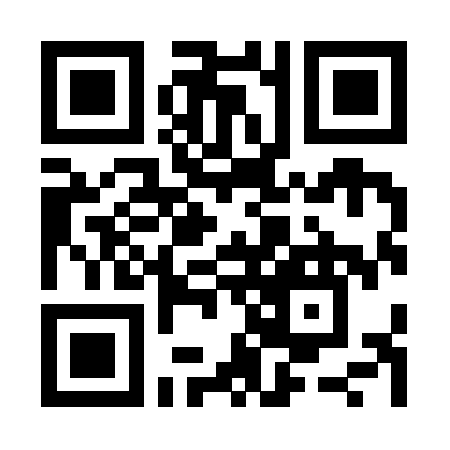
\includegraphics[scale=0.4]{pics/qr_Laplace.eps} 
}

$$ L \left [ f(t) \right] = \tilde{f}(s) = \int_{0}^{\infty}f(t)e^{-st}dt $$

где $s$ параметр пространства Лапласа соответствующий времени

Решение для бесконечно малого радиуса скважины в пространстве Лапласа будет иметь вид

\begin{equation}  \label{eq:laplace_solution_1}
	\tilde{p}_D(s) = \frac{1}{s} K_0 \left( r_D \sqrt s  \right) 
\end{equation}

решение для конечного радиуса скважины \cite{Everdingen_1949}

\begin{equation} \label{eq:laplace_solution_2}
	\tilde{p}_D(s) = \frac{K_0 \left( r_D \sqrt{s}  \right) }{ s \sqrt{s} K_1 \left( \sqrt s  \right)  }
\end{equation}

где 

$K_0$, $K_1$ - модифицированные функции Бесселя;

\marginpar{
	\href{https://qrgo.page.link/hkh7x}{модифицированные функции Бесселя} 
	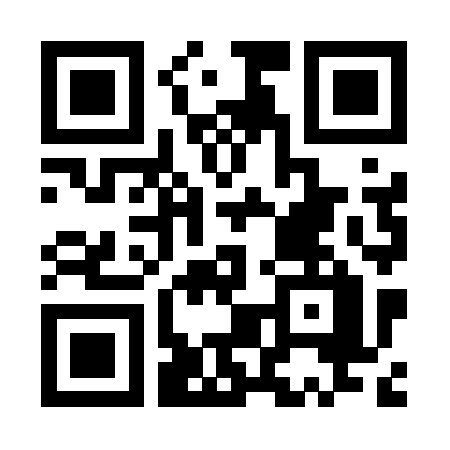
\includegraphics[scale=0.4]{pics/qr_Bessel.eps} 
}

$s$ - переменная пространства Лапласа;

$\tilde{p}_D(s)$ - изображение функции ${p}_D$ в пространстве Лапласа;

$r_D$ - безразмерный радиус скважины.

\

Перевод решения из пространства Лапласа в обычное пространство не всегда возможен аналитически. В современных условиях перевод делается численно с использованием компьютеров, что позволяет строить и исследования решения уравнения фильтрации при различных условиях. 

Широко распространено применения алгоритма Стефеста для численного обратного преобразования Лапласа. 

\subsubsection{Расчет в Unifloc VBA}

Следующие функции реализованы в Unifloc VBA

\begin{verbatim}
	transient_pd_radial
	transient_pwf_radial_atma
\end{verbatim}	

Описания функций и из аргументов можно найти в руководстве пользователя  Unifloc VBA



\section{Учет влияния ствола скважины}
Часто управление дебитом скважины производится на поверхности -- за счет регулировки на скважинной арматуре. При этом, например, перекрытие потока на скважинной арматуре не сразу приведет к прекращению притока из пласта на забое скважины. Для скважины оснащенной насосом со свободным динамическим уровнем приток из пласта будет продолжаться пока не заполнится затрубное пространство скважины. Для фонтанирующей скважины с пакером тот же эффект, хотя и заметно менее выраженный будет наблюдаться из за высокой сжимаемость газожидкостной смеси в стволе скважины. 

Эффект различия скоростей изменения дебита жидкости на устье и забое называют эффектом влияния ствола скважины или эффектом послепритока (wellbore storage). Он часто встречается, оказывает большое влияние на качество исследования и обязательно должен учитываться при интерпретации и моделировании исследований.

Простейший вариант учета эффекта послепритока описывается с использованием постоянного коэффициента послепритока или коэффициента влияния ствола скважины $C_s$, определяющего "сжимаемость" жидкости в стволе скважины.

$$ C_s = - \frac{ \Delta V}{ \Delta p} $$

Для фонтанирующей скважины:

Изменение объема жидкости в стволе скважины происходит за счет сжимаемости жидкости:

$$ \Delta V = -c{V_w}{\Delta P} $$

$$ C_s = - \frac{ \Delta V}{ \Delta p} $$

Для фонтанирующей скважины, коэффициент ствола скважины:

$$ C_s =  c {V_w} $$

$ V_w $ - объем жидкости в стволе скважины  [м$^3$]
$c$ - сжимаемость жидкости или газожидкостной смеси в стволе скважины [1/атм]

%todo нужен пример расчета с числами для скважины с разными значениями давления - где газа много и мало, где пакер есть и пакера нет

Влияние ствола в механизированной скважине:

$$ C_s = - \frac{ \Delta V}{ \Delta p} $$
$$ {\Delta V} = A_{cas}{\Delta h} $$
$$ {\Delta P} ={ro g}{\Delta h}$$
$$ C_s =  \frac{ A_{cas}}{ \Delta p} $$

$ A_{cas}$ - площадь поперечного сечения затрубного пространства, [м$^2$]


$ {\Delta h}$ - изменение уровня жидкости в затрубном пространстве, [ м ]

Решение уравнения фильтрации с учетом скин-фактор и послепритока
Для решения линейного стока граничное условие соответствующее послепритоку с постоянным $C_s$ можно записать как

$$ \lim_{r_D \to 0} {r_D \frac{\partial p_D}{\partial r_D}} = -1 + \left. C_D \frac{\partial p_D}{\partial t_D} \right|_{t_D=1}$$

Предположим, что у нас имеется решение задачи запуска скважины с постоянным дебитом в прострастве Лапласа без учета скин-фактора и послепритока $\tilde{p}_D^{*}$. Где $s$ параметр пространства Лапласа соответствующий $t_D$.

Например для бесконечного пласта и скважины нулевого радиуса такое решение имеет вид: 

$$\tilde{p}_D^*(s) = \frac{1}{s} K_0 \left( r_D \sqrt s  \right) $$

Тогда решение с учетом скин-фактора и послепритока может быть выражено 

$$\tilde{p}_D(s) = \frac{s \tilde{p}_D^* + S}{s \left( 1+s C_D \left( s \tilde{p}_D^* + S \right)  \right)}   $$



%\subsubsection{Решение для постоянного забойного давления}
%
%\subsubsection{Решение для скважины с ГРП}
%
%Надо привести решение для скважины с ГРП
%
%\subsubsection{Решение для скважины с горизонтальной скважиной}
%
%Надо привести решение для горизонтальной скважины




\subsection{Решение для скважины в пласте с непроницаемой границей}
надо добавить мнимую скважину

Пусть скважина, представленная на рисунке, находится на расстоянии L от прямолинейной непроницаемой границы, через которую отсутствует поток жидкости.



Математическая задача о работе скважины, находящейся на каком-то расстоянии L от непроницаемой прямолинейной границы, может быть рассмотрена как  работа двух скважин - данной и воображаемой, в данной случае добывающей, находящейся на расстоянии 2L от рассматриваемой. Воображаемая скважина работает с той же производительностью, что и фактическая скважина. Рассмотрение работы двухскважинной системы как аналога работы одной скважины с границей в пласте базируется на том, что равновесие двух рядом находящихся одинаково работающих скважин может наступить только при условии, что через линию, проходящую между скважинами и равноотстоящую от них, нет потока (то есть, градиент давление вдоль этой линии равен нулю). Таким образом можно записать работу двух скважин в бесконечном пласте в виде:

$$ P_{пл} - P_c = - \frac{q_A \mu}{4\pi kh} \left( ln \frac{1,67 \mu m c_t r_c^2}{kt}-2S \right)- \frac{q_B \mu}{4\pi kh} Ei \left( \frac{1,78 \mu c_t m \left(2L\right)^2}{4kt} \right)$$

Здесь также можно отметить, что в воображаемой скважине не принят во внимание скин - фактор, так как рассматривается влияние этой скважины на работу фактической скважины, находящийся на большем расстоянии от нее. 



Решение для скважины в пласте с границей постоянного давления 
Тут тоже надо добавить мнимую скважину и описать пример построения решения


\subsection{Другие применения принципа суперпозиции}
также можно добавить ряд других примеров

%скважине в секторе с двумя границами
%скважине в замкнутой области с несколькими границами 
%скважина с ГРП - метод источников
%группа скважин взаимодействующих между собой
%горизонтальная скважина
%горизонтальная скважина с ГРП

